\chapter[Abundances of methane isotopologues at the Potato
Hills gas field, southeastern
Oklahoma]{Abundances of methane isotopologues at the \\Potato
	Hills gas field, southeastern
	Oklahoma}\label{dx:A}
\chaptermark{Potato Hills}

\begin{abstract}
	\noindent Wells in the Potato Hills region of the Ouachita Mountains, southeastern
	Oklahoma, produce dry natural gas from fractured sandstone units of the
	Pennsylvanian-age Jackfork Group. Previous carbon- and hydrogen-isotope
	measurements of the C\textsubscript{1}--C\textsubscript{4} hydrocarbons
	of these gases revealed that methane is enriched in
	\textsuperscript{13}C and D relative to the C\textsubscript{2+}
	components \parencite{Seewald+Whelan_2005_AAPG-Origin-of-Petroleum}. This pattern of ``isotopic
	reversal'' is commonly-associated with high-maturity gases produced from
	unconventional deep-basin and shale reservoirs \parencite[e.g.,][]{Burruss+Laughrey_2010_OG,Tilley++_2011_AAPGB}, and suggests that gases
	produced in the Potato Hills may have a deep source. However, because of
	the structural complexity of this region, identifying potential source
	rocks and migration pathways has been difficult.
	
	Here, we report additional constraints from tunable infrared laser
	direct-absorption spectroscopy analyses \parencite[see][]{Ono++_2014_AC} of the
	abundance of \textsuperscript{13}CH\textsubscript{3}D (a methane
	``clumped'' isotopologue) in natural gas from the Potato Hills field.
	The measured isotopic signatures are similar across five different wells
	drilled to 1.8--2.3 km depth, suggesting both a common source for the
	methane in these gas samples, and preservation of the C--H bond across
	this \textgreater{}50 km\textsuperscript{2} reservoir system.
	
	Our measurements suggest an apparent \textsuperscript{13}C--D isotopic
	temperature of \textasciitilde{}150 ± 30~°C for methane from the Potato
	Hills field. Application of a model for isotopic exchange suggests that
	migration of thermogenic gases generated at temperatures below 200~°C
	should not result in any detectable reordering of the C--H bonds in
	methane. We discuss uncertainties in the model calibration and
	implications for the preservation of clumped isotopic signatures in
	methane. Results are further interpreted in the context of the regional
	geology to highlight potential implications for natural gas occurrences
	in the Ouachita overthrust belt and beyond.
\end{abstract}

\vspace*{\fill}

\noindent \rule{\textwidth}{0.4pt}\\

{\small
	
	\noindent Preliminary data from this chapter were presented in a talk at the
	24\textsuperscript{th} Annual V.M. Goldschmidt Conference in Sacramento,
	California, USA, June 2014. \\
	
	\noindent This work was done in collaboration with Jeff Seewald (and indirectly,
	Jean Whelan) of WHOI with oversight from Shuhei Ono.
	
}

\clearpage

\section{Introduction}\label{introduction-3}


\begin{sidewaysfigure}
	%	\centering
	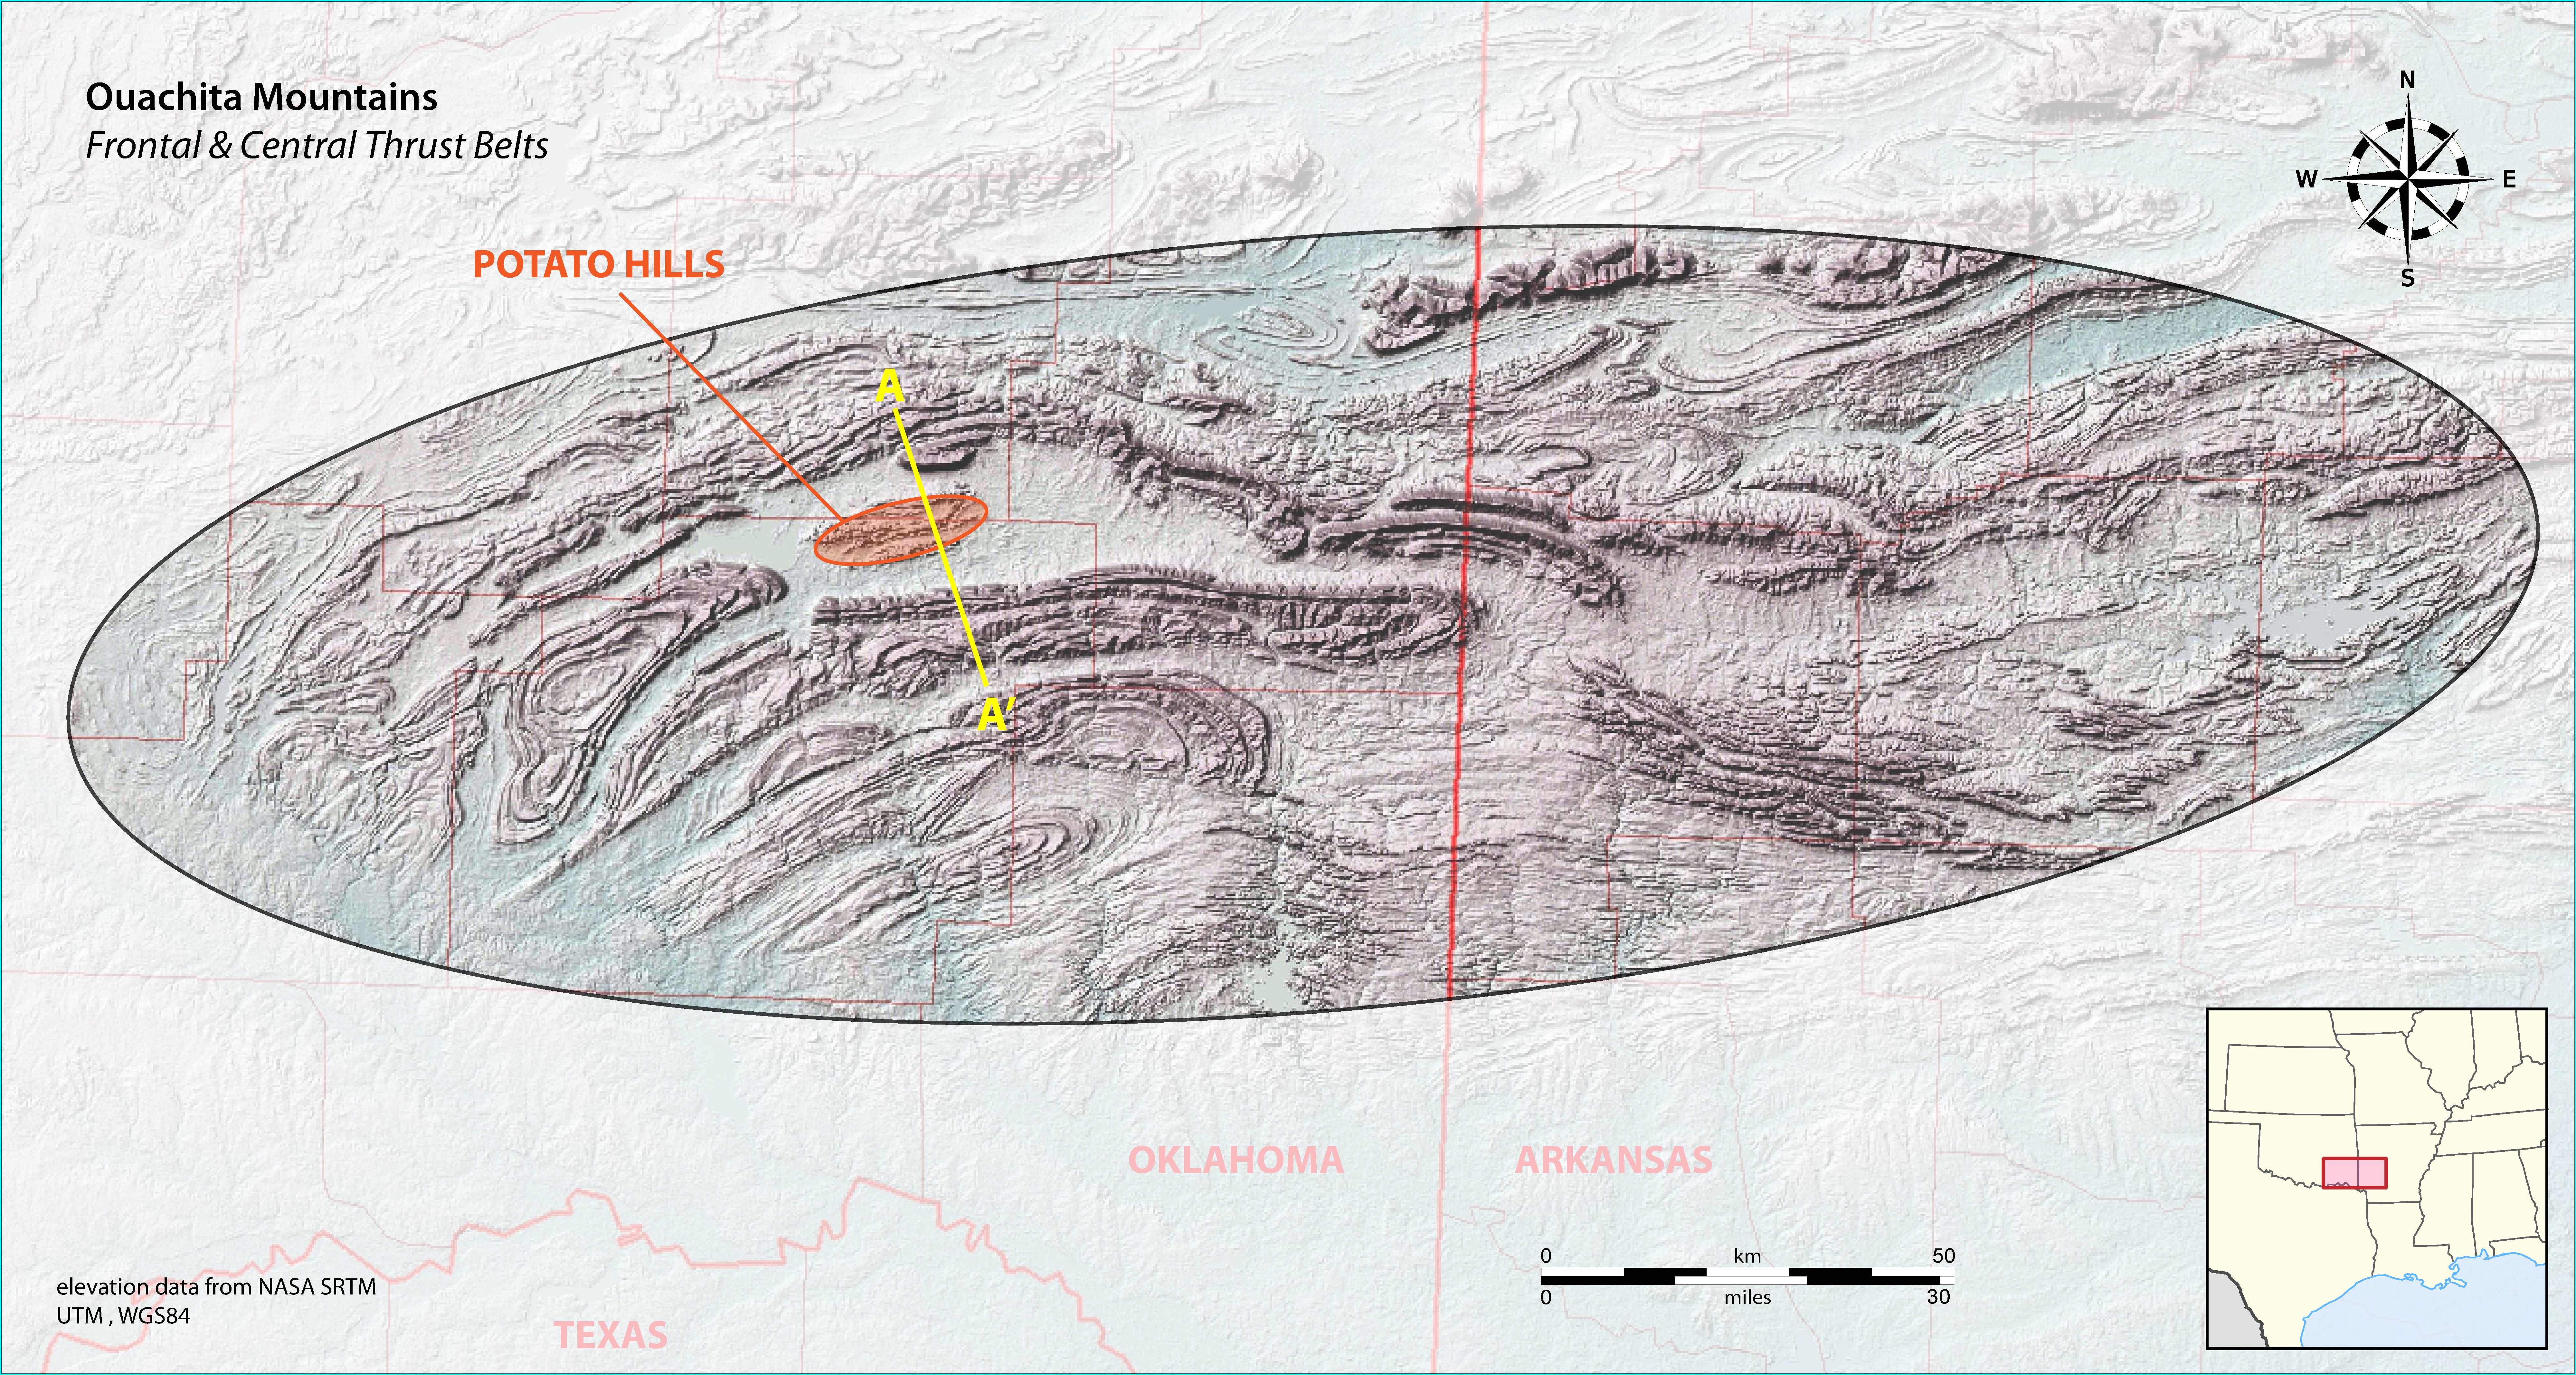
\includegraphics[width=\textwidth]{figures/FigA.1.pdf}
	\caption[Map of the frontal and central Ouachita thrust belt]{Relief map of the frontal and central Ouachita
		overthrust belt, southeastern Oklahoma and western Arkansas, USA.}
	\label{fig:A:1}
\end{sidewaysfigure}
\begin{sidewaysfigure}
	%	\centering
	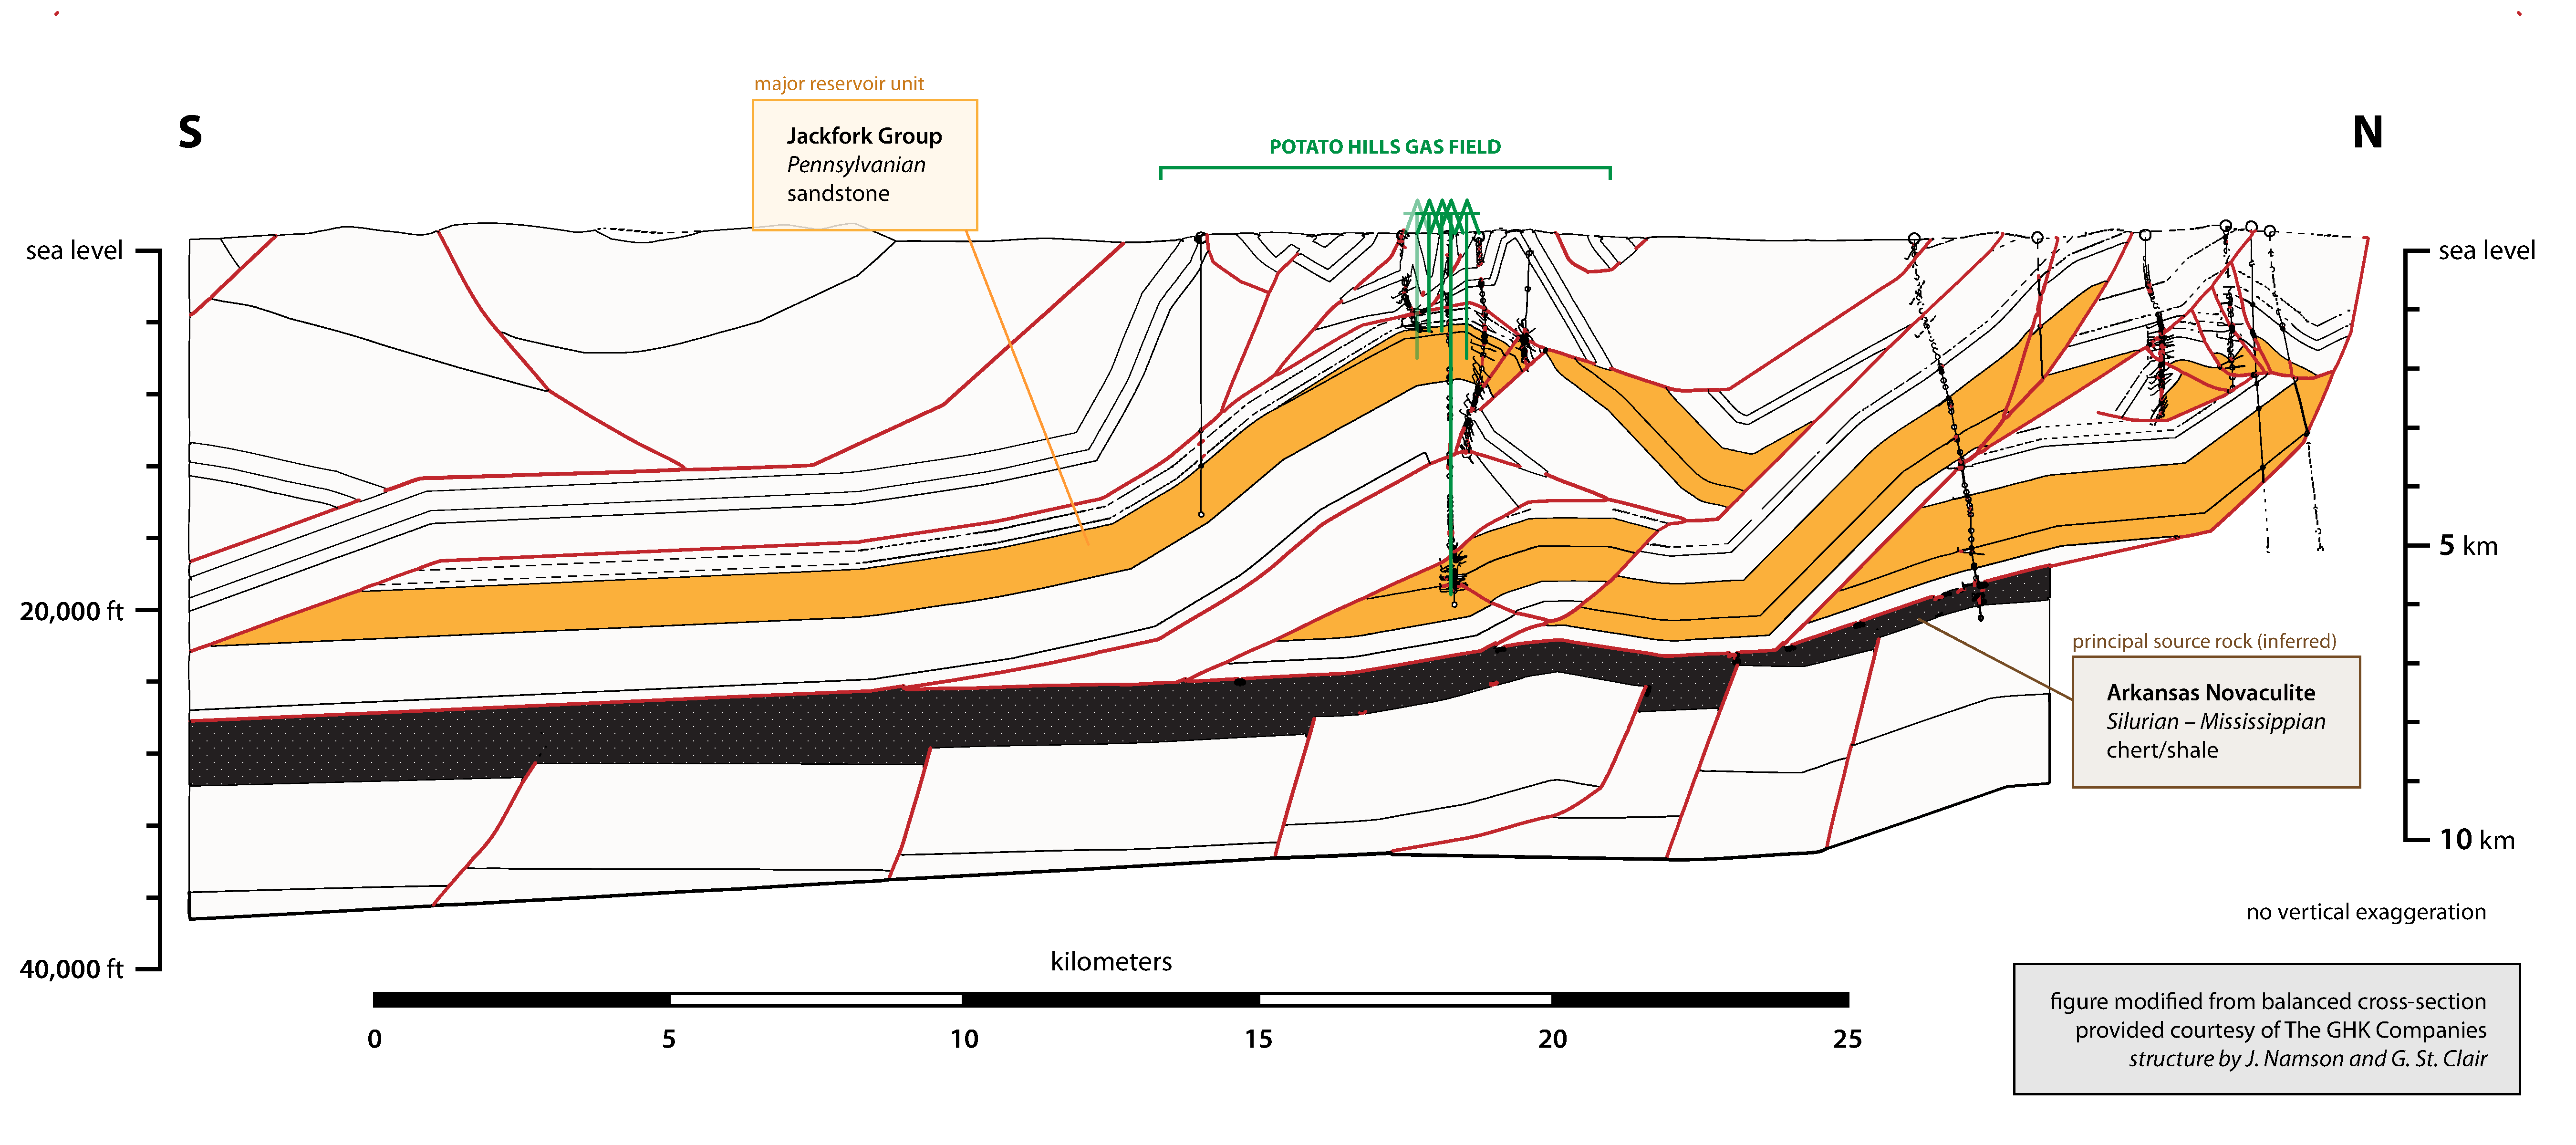
\includegraphics[width=\textwidth]{figures/FigA.2.pdf}
	\caption[Structural cross-section through the Potato Hills]{Balanced geologic cross-section through the Potato
		Hills for A--A$'$ (\autoref{fig:A:1}). The original cross-section on which this figure
		is based was provided courtesy of The GHK Companies. Structural
		interpretation was by J. Namson and G. St.\ Clair. Reservoir sands and
		presumed source are highlighted in orange and black, respectively.
		Faults are highlighted in red. Projections of studied wells onto the
		cross-section are shown in green.}
	\label{fig:A:2}
\end{sidewaysfigure}

The subject of this study is produced gas sampled from the Potato Hills
gas field in southeastern Oklahoma. The Potato Hills is located in a
structurally complex region of the Ouachita Mountains within the
frontal/central thrust belt (\autoref{fig:A:1}).\footnote{The name is apparently
	due to the resemblance of the unevenly-eroded outcrops of the
	fractured Bigfork Chert (late Ordovician) to the knobby mounds of a
	potato garden:
	\url{http://www.ghkco.com/contact/index.php?page=Potato\_Hills}} Wells in
the Potato Hills gas field produce from repeated (subthrusted) intervals
of the fractured and porous sandstones of the Pennsylvanian-age Jackfork
Group (\autoref{fig:A:2}). The field was discovered in the 1960s, but produced little gas and was soon abandoned. Several decades later, The GHK Companies realized the Jackfork play concept and established several
dozen wells in the area beginning in 1997. The Potato Hills is one of
the most significant recent conventional gas discoveries in Oklahoma
\parencite{Boyd_2005_OKGN}, and has produced \textgreater{}300 BCF
(\textasciitilde{}50 MMBOE) of gas.

Major tectonism and mountain building coincided with the collision of
the South American Plate with the North American continent (Laurentia)
during the late Pennsylvanian and early Permian (ca.\ 300~Ma, the
Ouachita orogeny) \parencite{Hatcher++_1989}. During the approach and leadup
to the eventual collision, large deposits of Silurian to
Mississippian-age sediments derived from North American rivers filled
the ocean basin between the two continents. In the Ouachitas, these
sediments are known as the Arkansas Novaculite, an organic-rich (up to
4\% TOC in drill cores, and possibly up to 15\% originally), mixed
shale-chert unit.\footnote{The perhaps more familiar Woodford Shale (to the
north of the Ouachitas, in the Arkoma Basin) is syndepositional to the
Arkansas Novaculite. The Arkansas Novaculite is the basinward extension
of the Woodford Fm.\ \parencite{Houseknecht++_2014_AAPGB}.} While no data from
source rocks in the Potato Hills could be located, the Arkansas
Novaculite elsewhere in the Ouachitas contains predominantly gas-prone
Type III kerogen \parencite{Curiale_1981_thesis}.

Gases from the Potato Hills are dry (\textgreater{}95\%
C\textsubscript{1}/$\big\sum\!$C\textsubscript{1--4}) and express a
partially-reversed isotopic trend in which the CH\textsubscript{4} is
enriched in \textsuperscript{13}C and D relative to C\textsubscript{2}
and higher hydrocarbon gases \parencite{Seewald+Whelan_2005_AAPG-Origin-of-Petroleum}. This partial
reversal is observed in all wells studied, with the exception of the
deep (6.3~km) Mary 2-34 well which produces gases with reversed
δ\textsuperscript{13}C but normal δD (i.e., δD of CH\textsubscript{4}
\textless{} δD of C\textsubscript{2}) (Seewald and Whelan, unpublished
data). Notably, the δD signature of CH\textsubscript{4} is highly
uniform amongst all studied gases (see \autoref{tab:A:1} for a partial listing),
including the deep well.

These gases were studied for two reasons: (\emph{i}) they were samples
of opportunity that were associated with an already-existing dataset
comprising analyses of the chemical and isotopic composition of produced
gases, concentrations of aliphatic acids in coproduced formation waters,
and cultivation-based and culture-independent microbiological data
(Seewald, Whelan, and Sievert, unpublished data); and (\emph{ii}) to
test if migrated thermogenic gases that accumulated in low temperature
reservoir units and were retained over timescales of millions of years
would record primary clumped isotopologue signals.

\section{Methods}\label{methods-2}

\subsection{Samples}\label{samples}

Samples were retrieved from a dusty Pelican case underneath a desk in
Fye 142A at the Woods Hole Oceanographic Institution in October of 2013.

The studied samples were collected from the wellhead in the early 2000's
by GHK in stainless steel cylinders equipped with high-pressure valves,
and furnished to J.\ Seewald and J.\ Whelan for chemical and isotopic
analyses. Data on carbon and hydrogen isotopes of CH\textsubscript{4}
obtained circa 2003 at WHOI \parencite{Seewald+Whelan_2005_AAPG-Origin-of-Petroleum} are shown in
\autoref{tab:A:1}.

There was no evidence of compromised sample integrity when the samples
were examined in 2013--2014. All gas cylinders studied contained gas at
high pressure, and analyses of δ\textsuperscript{13}C and δD in 2014
yielded data that matched those obtained ten years earlier (\autoref{tab:A:1}).

One sample (Mary 2-34) was later mistakenly shipped to UCLA, where it resided for a year.  The missing sample was located and returned to MIT with the help of I.E. Kohl.  All samples are now safely back at WHOI.

\subsection{Analysis}\label{analysis}


\begin{figure*}
	\centering
	\includegraphics[width=0.85\textwidth]{figures/FigA.3.pdf}
	\captionsetup{format=myformat}	% hrule beneath caption
	\caption[Histogram of isotopologue ratios from a single measurement run]{Histogram of log-delta values (referenced to an
		arbitrary set of isotopologue ratios) for CH\textsubscript{4} purified
		from the Hicks \#1 cylinder, measured on the TILDAS during a single
		sample run (\textasciitilde{}10 hours). Here, \emph{n} represents the
		number of measurement cycles made during this run; in each measurement
		cycle, samples are measured for 100 seconds, and each sample measurement
		is bracketed by measurements on the reference gas.}
	\label{fig:A:3}
\end{figure*}


These samples were the first ``real'' samples ever measured for clumped
isotopologues of methane at MIT. At the time these data were obtained,
the Methane PrepLine (\autoref{dx:C}) had not yet been built, so sample
purification was done manually in a cryogenic vacuum line interfaced
with a gas chromatograph supplied with helium carrier and a handmade
packed column held near ambient temperature.

Analyses of the methane clumped isotopologue
\textsuperscript{13}CH\textsubscript{3}D were made with a prototype
tunable infrared laser direct absorption spectrometer (TILDAS) developed
by Aerodyne Research, Inc.\ (Billerica, MA) and housed in the Hardcore
Stable Isotope Laboratory at MIT. Analytical procedures are documented
in \textcite{Ono++_2014_AC}. A histogram of isotopologue data obtained on
multiple measurement cycles (\emph{n} = 36) for one sample is shown in
\autoref{fig:A:3}.


\section{Results \& Discussion}\label{results-discussion}

\subsection{Preservation potential of clumped isotopologue
	temperatures in migrated thermogenic
	gases}\label{preservation-potential-of-clumped-isotopologue-temperatures-in-migrated-thermogenic-gases}


\begin{table}
	\caption[Isotopic composition of methane from the Potato Hills
	gas field]{Isotopic composition of methane from the Potato Hills
		gas field. Data taken at WHOI soon after sampling \parencite{Seewald+Whelan_2005_AAPG-Origin-of-Petroleum} are compared with data obtained on the same cylinders measured at
		MIT (via TILDAS) one decade later.  All isotope values are in permil (‰).}
	\label{tab:A:1}
	\centering
	\begin{threeparttable}
		\begin{tabular}{l c c cc l ccc c}
			\toprule
			& & & \multicolumn{2}{c}{WHOI (c.\ 2003)} & & \multicolumn{3}{c}{MIT (January 2014)}\tabularnewline
			\cmidrule{4-5} \cmidrule{7-9}
			Well Name & TD (km) & \emph{T}\textsubscript{res} (°C) &
			δ\textsuperscript{13}C & δD & & δ\textsuperscript{13}C & δD &
			Δ\textsuperscript{13}CH\textsubscript{3}D\,\textsuperscript{a} &
			\emph{N}\tabularnewline
			\midrule
			Cedar Creek & 1.78 & 45 & $-$38.1 & $-$134 & & $-$38.4 & $-$136.8 & 3.10 ± 0.25 &
			2\tabularnewline
			Stevens \#1 & 1.86 & 50 & $-$36.9 & $-$139 & & $-$38.1 & $-$136.6 & 3.08 ± 0.37 &
			3\tabularnewline
			Hicks \#1 & 2.29 & 51 & $-$37.0 & $-$135 & & $-$38.2 & $-$136.8 & 3.17 ± 0.20 &
			3\tabularnewline
			Koopmans \#1 & 2.20 & 53 & $-$39.5 & $-$133 & & $-$40.9 & $-$135.3 & 3.30 ± 0.12 &
			5\tabularnewline
			Mary 2-34 & 6.29 & 126 & $-$31.2 & $-$136 & & $-$32.5 & $-$139.7 & 2.94 ± 0.20 &
			5\tabularnewline
			\bottomrule
		\end{tabular}
		{\small TD, total depth; \emph{T}\textsubscript{res}, reservoir temperature; and
		\emph{N}, number of independent replicate purifications and
		measurements.}
		\begin{tablenotes}
			\item[a] The uncertainty on the
			Δ\textsuperscript{13}CH\textsubscript{3}D incorporates propagated 95\%
			confidence intervals calculated assuming a normal distribution, and also
			includes the error on Δ\textsuperscript{13}CH\textsubscript{3}D of AL1.
		\end{tablenotes}
	\end{threeparttable}
\end{table}


Drilled depths and measured reservoir temperatures shown in \autoref{tab:A:1} were
obtained from public records on the website of the Oklahoma Corporation
Commission. Comparison of bottom-hole temperatures to depth for 16 wells
in this area (data from GHK, not shown) suggests a local geothermal
gradient between 15 and 25~°C per kilometer, consistent with the
reported reservoir temperatures and known depths of those reservoir
intervals (\autoref{fig:A:2}).

The Δ\textsuperscript{13}CH\textsubscript{3}D values of gases from all
wells were identical within error, although the deeper Mary 2-34 sample
may carry a slightly lower value (by \textasciitilde{}0.2‰). Samples
yielded geologically-realistic apparent equilibrium temperatures of
\textasciitilde{}150 ± 30~°C (\autoref{fig:A:4}).

To test if these signals might be primary (i.e., if
Δ\textsuperscript{13}CH\textsubscript{3}D values are the same as those
these gases had at the time of their expulsion from the source rock), we
modeled the kinetics of hydrogen isotopic exchange (\autoref{fig:A:4}). This model
uses the rate of CH\textsubscript{4}--H\textsubscript{2}O isotopic
exchange reported by \textcite{Koepp_1978}, and assumes that rates scale with
temperature according to the Arrhenius equation. These rates are subject
to large uncertainty; this is discussed in more depth in \autoref{ch:3} and
in reviews by \textcite{Schimmelmann++_2006_AREarth,Sessions++_2004_GCA}.
Furthermore, the model assumes that
Δ\textsuperscript{13}CH\textsubscript{3}D values will not reset unless
CH\textsubscript{4} exchanges with H\textsubscript{2}O---that is,
homogenous isotope exchange is implicitly excluded as a mechanism for
isotopologue reordering. It is unknown if mineral surfaces encountered
by the hydrocarbons may serve as catalysts for homogenous isotope
exchange \parencite{Shipp++_2014_PNAS}; this would lower the activation energy
and allow isotopic reordering at lower temperatures than indicated.


\begin{figure*}
	\centering
	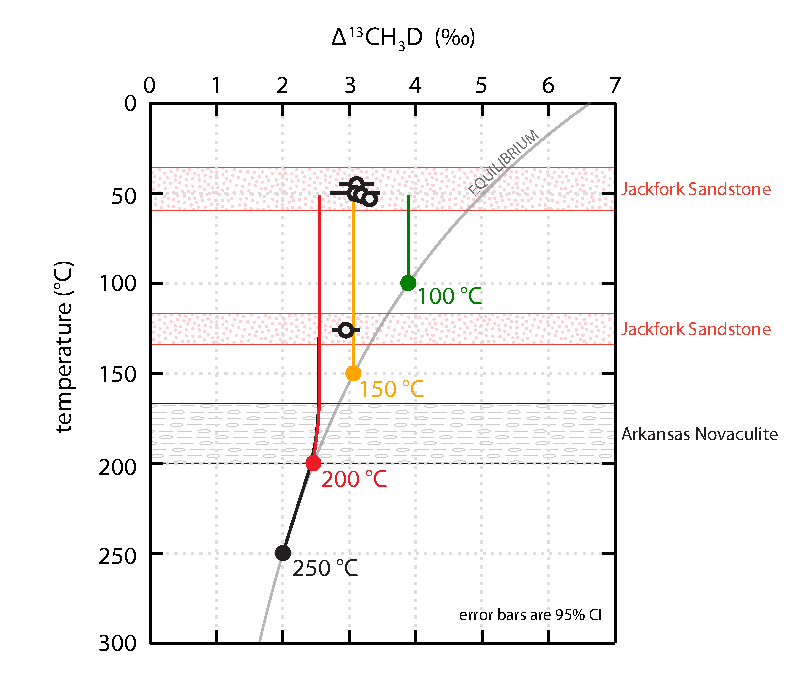
\includegraphics[width=0.9\textwidth]{figures/FigA.4.pdf}
%	\captionsetup{format=myformat}	% hrule beneath caption
	\caption[Cooling model for migrated gases at Potato Hills]{Model of migrating gases. The colored points on the
		model curves represent initial compositions of natural gases that were
		generated at 350~Ma at temperatures from 100 to 250~°C. The gases were
		assumed to be carrying Δ\textsuperscript{13}CH\textsubscript{3}D values
		equal to those expected for equilibrium at these starting temperatures.
		These model gases then were cooled at a rate of 10~°C per Myr until 330~Ma, at which cooling ceased. Curves show the predicted clumped
		isotopologue compositions of gases (\emph{x}-axis) with temperature (\emph{y}-axis).
		Clumped isotopologue reordering was treated as a first-order reaction
		obeying the Arrhenius equation, with pre-exponential factor
		\SI{6.1e9}{\second^{-1}} and activation energy
		209 kJ mol\textsuperscript{$-$1} \parencite[estimated from the data of][]{Koepp_1978}. Data from \autoref{tab:A:1} are shown for comparison. The equilibrium
		curve is that of \textcite{Wang++_2015_S}, for which the equation is listed in
		\autoref{dx:C} (\autoref{eqn:C:equilibrium}).}
	\label{fig:A:4}
\end{figure*}


Migration from source to reservoir is generally thought to be fast
relative to the process of petroleum generation in the source rock
\parencite{England++_1991_AAPG-SV}. A conservative estimate of rates of cooling
during fluid migration was applied (10~°C per Myr). The model results
suggest that isotopic reordering of C--H bonds within
CH\textsubscript{4} is sluggish or non-detectable on timescales relevant
to petroleum migration at temperatures below 200~°C (\autoref{fig:A:4}). This
suggests that if methane generation occurred in the source rocks at
\textless{}200~°C, the signature the methane carried at generation would
have been preserved during its residence in the shallower traps. The
deeper traps may have exceeded this temperature, however (see \autoref{c-h-isotopes-and-the-filling-or-fate-of-fluids-in-the-potato-hills-reservoirs}).
The uniformity of δD but variation in δ\textsuperscript{13}C with depth
indicates that hydrogen exchange has occurred, either by
CH\textsubscript{4}--H\textsubscript{2}O directly, or more likely,
between precursor kerogen and water \parencite{Clayton_2003_IMOG}. Supporting this is
evidence that the Arkansas Novaculite in wells in the vicinity of the
Potato Hills may have reached very high maturities (vitrinite
reflectance \textgreater{}4\% R\textsubscript{o}) \parencite{Guthrie++_1986_AAPGB}.

\subsection{C \& H isotopes and the filling or fate of fluids in the
	Potato Hills
	reservoirs}\label{c-h-isotopes-and-the-filling-or-fate-of-fluids-in-the-potato-hills-reservoirs}

With the exception of the deep well (Mary 2-34), all
δ\textsuperscript{13}C values for methane are quite homogeneous at
around $-$38‰. The methane from Mary 2-34 is characterized by a distinctly
\textsuperscript{13}C-enriched value of $-$32‰, whereas δD is nearly
identical to those of the wells which produce from the shallower
reservoir interval.

Because δ\textsuperscript{13}C values of methane tend to increase with
increasing thermal maturity \parencite{Hunt_1996}, the marked
\textsuperscript{13}C-enrichment in the Mary 2-34 sample suggests that
the deeper reservoir interval was filled by gases that were, on average,
generated at higher temperatures or at a later stage than the gases
which accumulated and were retained in the shallower structural traps.
Several scenarios are possible: (\emph{i}) the shallower trap filled
first, followed later by charging of the deeper trap by more mature
gases; (\emph{ii}) charging of the deeper trap occurred first with enough gas to
fill the deeper reservoir, and spilled over such that the shallower
unit received a vicarious, \textsuperscript{13}C-depleted charge; or 
(\emph{iii}) C\textsubscript{2+} gases in the deeper reservoir have
experienced thermal breakdown or stepwise oxidation such that the
originally \textsuperscript{13}C-depleted signature of
CH\textsubscript{4} has been diluted by heavier carbon-isotope signals
derived from C\textsubscript{2+}.

Interpretations of mapped and extrapolated fault geometries suggest that
thrusting in the frontal and central thrust belts of the Ouachitas
occurred in a break-forward style \parencite{Miser_1929_OGS,Cemen++_2002}.
This implies that crustal shortening, accommodated by development of the
imbricate thrust sheet, was characterized by the formation of new
thrusts underneath older thrusts as the units in the hanging wall moved
forward along the detachment \parencite{Boyer+Elliott_1982_AAPGB,Shaw++_1999_GSAB}. If break-forward thrusting was responsible for the development of
the structural traps of the Potato Hills field, the first scenario may
well be possible.

No information is available to evaluate the second scenario
(fill-to-spill and tertiary migration).

The third scenario is supported by observations of high concentrations
(tens of millimolar) of acetic acid in reservoirs of the Potato Hills
field (Seewald and Whelan, unpublished data). Such high concentrations
of short-chain carboxylic acids are not atypical of oilfield waters
\parencite{Kharaka++_1973_GCA,Willey++_1975_GCA,Carothers+Kharaka_1978_AAPGB,Seewald_2003_N}, and may reflect stepwise oxidation of
C\textsubscript{2+} alkanes to carboxylic acids during residence of the
hydrocarbon fluids in the deep reservoirs \parencite{Shock_1988_G,Seewald_2001_GCA_model}.
Considering that temperatures in the lower reservoir exceed 120~°C
currently, and were likely much higher in the past given that several
kilometers of overburden may have eroded since the Permian \parencite{Godo++_2011_AAPG-ACE}, decomposition of C\textsubscript{2+} alkanes at depth may also
explain features of the isotopic reversals observed \parencite{Burruss+Laughrey_2010_OG,Tilley++_2011_AAPGB,Zumberge++_2012_MPG,Tilley+Muehlenbachs_2013_CG}.

\section*{Acknowledgments}

I thank Jeff Seewald for sharing his samples and data. The GHK Companies
provided much of the background data, the funding for visits to the
producing wells by J. Seewald, J. Whelan, and S. Sievert, and support
for analyses performed at WHOI in the early 2000s. My studies on the
Potato Hills were conducted while under the support of the NDSEG
Fellowship program.








